%\documentclass{proc}
%\usepackage{graphicx}


\documentclass[10pt]{article}
\usepackage{lipsum}% http://ctan.org/pkg/lipsum
\usepackage{calc}% http://ctan.org/pkg/calc
\usepackage[
  a4paper,%
%  textheight={47\baselineskip+\topskip},%
  textwidth={\paperwidth-126pt},%
  footskip=75pt,%
  marginparwidth=0pt,%
  top={\topskip+0.75in}]{geometry}% http://ctan.org/pkg/geometry
\usepackage{fancyhdr}% http://ctan.org/pkg/fancyhdr
\usepackage{graphicx}
\usepackage[]{algorithm2e}
\usepackage{url}
\usepackage{float}
\usepackage{textcomp}
\usepackage{amsmath}
\usepackage{graphicx}
%\usepackage{babel}

\pagestyle{fancy}
\fancyhead{} \fancyfoot{}% Clear header & footer
\fancyhead[C]{MATH-454 : Semester projects}% Set centered header
\fancyfoot[C]{\thepage}% Set centered footer
\renewcommand{\headrulewidth}{0.5pt}% Add header rule

% Titling
\author{ me }% Your author
\date{ \today }% Your date
\makeatletter
% Definition of proc.cls' \maketitle:
\def\@maketitle{% 
  \vbox to 2.25in{%
    \hsize\textwidth
    \linewidth\hsize
    \vfil
    \centering
    {\LARGE \@title \par}
    \vskip 2em
    {\large \begin{tabular}[t]{c}\@author \end{tabular}\par}
    \vfil}}
\makeatother

\begin{document}

\title{\textbf{Parallel and High Performance Computing} \\\textbf{MATH-454}\\\textbf{PROJECTS}}
%\author{Vincent Keller \\Nicolas Richart\\Nicola Varini}
\author{Vincent Keller \\Nicolas Richart}

\maketitle

%\begin{abstract}
%The abstract text goes here.
%\end{abstract}

\section{Introduction}

\begin{itemize}
	\item{$\sim$ 40 hours of personal and individual work}
	\item{We suggest 3 subjects}
	\item{\textbf{PhD students have the possibility to propose their own projects}}
	\item{Two implementations must be delivered : \begin{enumerate} \item{MPI (OpenMP/hybrid/MPI-IO are a plus)}\item{CUDA}\end{enumerate}}
	\item{C/C++ or Fortran are accepted}
	\item{All the deliverables have to be handed in via the Moodle page}
\end{itemize}


\subsection{Important dates}

\begin{center}
\begin{tabular}{ | l | l |}
\hline
\textbf{Deliverable} & \textbf{Due date} \\
\hline
Fixing topic & May 4, 2020 \\
\hline
\textit{Theoretical Analysis (optional)} & \textit{May 25, 2020} \\
\hline
Final Report & June 8, 2020 \\
\hline
Presentation's slides & June 15, 2020 \\
\hline
Exam (15' pres + 5' Q\&A) &  TBD \\
\hline
\end{tabular}	
\end{center}

\section{The projects}

\subsection{Conjugate Gradient Method (CG) for solving Ax = b}

\begin{figure}[H]
\center

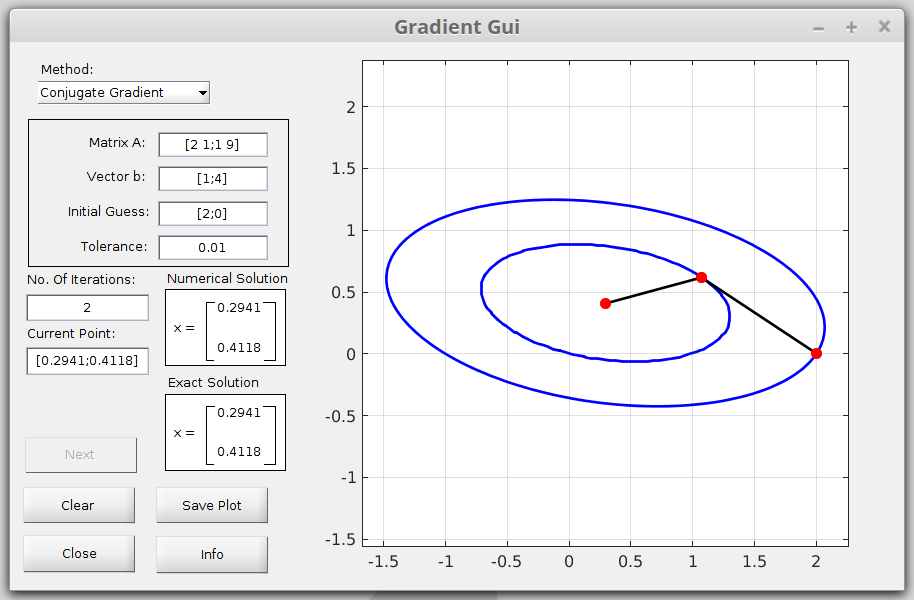
\includegraphics[width=118mm]{cg}
\caption{screenshot from http://m2matlabdb.ma.tum.de}
\end{figure}

\textbf{Problem description}
\\

\begin{itemize}
	\item{Solve $Ax = b$ with the ``iterative'' CG without pre-conditioning}
	\item{A is a full, real, symmetric, positive-definite matrix ($x^T A x > 0$. $\forall x \in \Omega$)}
	\item{CG generates a solution $x_k$ at iteration $k$ with $x_{k+1} = x_k + \alpha_k p_k$ where 
		\begin{itemize}
		\item{$p_k$ is the conjugate vector at iteration $k$ (or \textit{search direction})}
		\item{$\alpha_k$ is the step length at iteration $k$}
		\end{itemize}
	}
	\item{$r_k = b - A x_k$ is the residual}
	\item{$p_k$ is always conjugated with the previous $p_{k-1}$. i.e. define $\beta_k$'s such $\beta_k = \frac{r_k^T A p_{k-1}}{p_{k-1}^T A p_{k-1}} = \frac{r_k^T r_k}{r_{k-1}^T r_{k-1}}$}
\end{itemize}

\textbf{Basic sequential algorithm}
\\


\begin{algorithm}[H]
	\KwData{A,b,$x_0$}
	\KwResult{x such $Ax = b$}
	initialization:\\
	usually $x_0 = 0$\\
	$r_0 := b - A x_0$\\
	$p_0 = r_0$ \\
	$k := 0$\\
	\While{$||r_{k + 1}|| > 0$}{
	   $\alpha_k := \frac{r_k^T r_k }{ p_k^T A p_k}$ \\
	   $x_{k+1} := x_k + \alpha_k p_k$ \\
	   $r_{k+1} := r_k + \alpha_k A p_k$ \\
	   $\beta_k := \frac{r_{k+1}^T r_{k+1} }{ r_k^T r_k}$ \\
	   $p_{k+1} := - r_{k+1} + \beta_k p_k$ \\
	   $k := k+1$ \\	
	}
\end{algorithm}

A sequential code is available at : \url{https://c4science.ch/source/CG-PHPC/browse/master/}. Matrices are read in matrix market format. You can find matrices files on \url{https://sparse.tamu.edu/}. 


\subsection{N-Body Problem}

\begin{center}
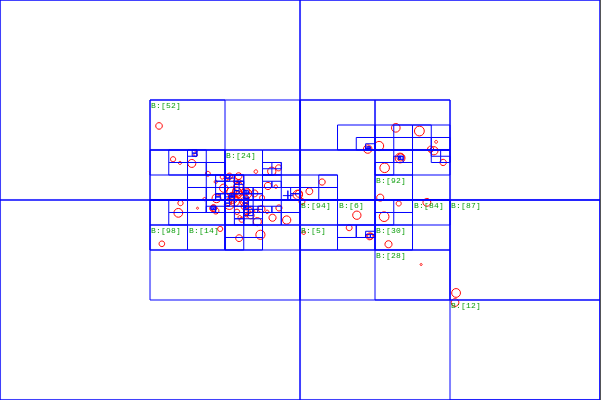
\includegraphics[width=118mm]{../../Day2/images/nbody.png}
\end{center}

\textbf{Problem description}
\\

The n-body problem aims at simulating a dynamical system of particles under the influence of physical forces. We'll restrain on the gravity field applied on celestial bodies:
$$
F_{ij} = \frac{G m_i m_j (q_j - q_i)}{||q_j - q_i||}
$$
where $G$ is the gravitational constant, $m_i$ and $m_j$ the masses of the $i$-th and $j$-th bodies and $q_i$ and $q_j$ their positions.
\\

\textbf{Possible algorithms}
\\

\begin{itemize}
	\item{\textbf{Particle-Particle Method} : this brute force algorithm will not be accepted (excepted for the CUDA implementation)}
	\item{octrees}
	\item{Particle-based mesh methods}
	\item{Fast Multipole}
\end{itemize}



\textbf{Important remarks}
\\

\begin{itemize}
	\item{3D}
	\item{non-uniform initial distribution must be tested to stress the application. You can easily modify your distribution by adding any massive object}
	\item{how to handle collisions and ``lost bodies in the far space''}
\end{itemize}

The test cases are read in the Gadget2 format (\url{https://wwwmpa.mpa-garching.mpg.de/gadget/}). 
\\

A sequential code is available on \url{https://c4science.ch/source/nbody-phpc}


\subsection{Shallow Water Wave Equation with a finite volume solver}

\begin{figure}[H]
\center

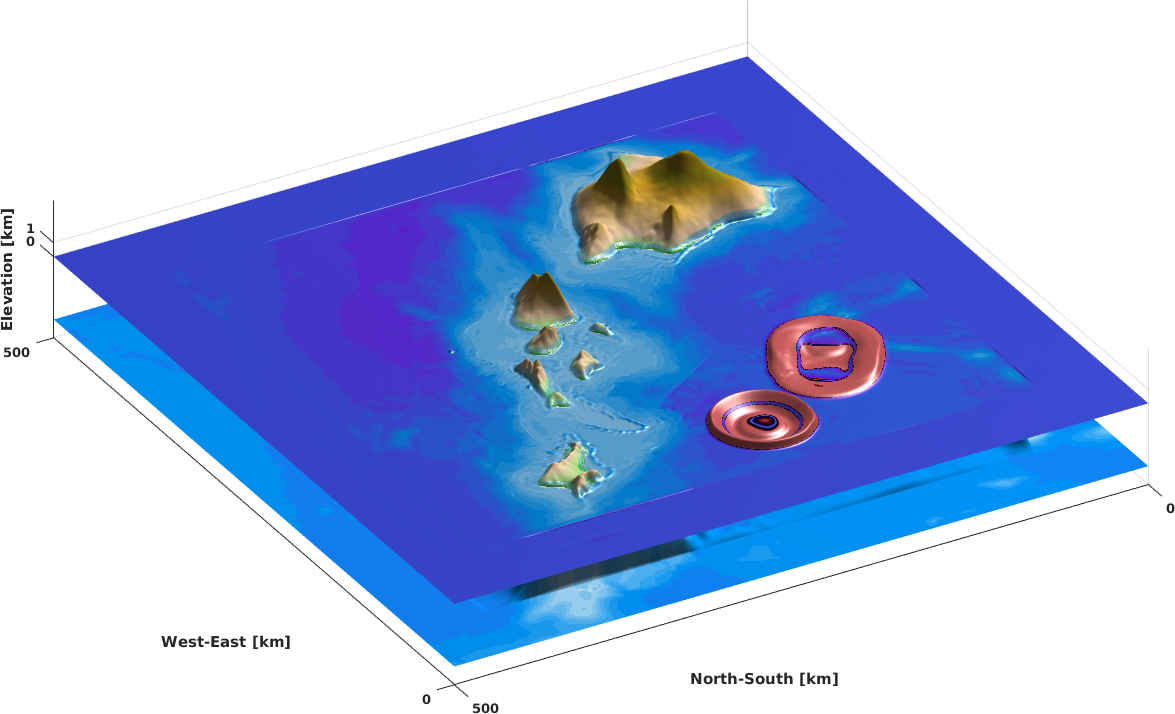
\includegraphics[width=118mm]{tsunami}
\end{figure}


An oceanographic researcher has written a simple predictive tool to
simulate Tsunamis as they move over oceans and overflow land. Unfortunately,
the Matlab code is prohibitively slow! Running the high-resolution
simulation takes several hours on a workstation. You are asked to
write new code that can simulate the Tsunami much faster. Use the
new techniques that you have learned in MATH454 and the computational
resources available at SCITAS so to help the researcher. The Matlab
code and data is available in the project folder, and below you will
find a short introduction to the model and the mathematics. 

\subsubsection*{Introducing the Model}

The shallow water wave equation is a non-linear hyperbolic system
of coupled partial differential equations often used to model various
wave phenomenons. Simulation of ocean waves, river flows, hydraulic
engineering and atmospheric modeling are among the many areas of application.
The researcher has used the two dimensional version of the equations
along with a right hand side source term as his model
\begin{align*}
 & \begin{cases}
h_{t}+\left(hu\right)_{x}+\left(hv\right)_{y}=0\\
\left(hu\right)_{t}+\left(hu^{2}+\frac{1}{2}gh^{2}\right)_{x}+\left(huv\right)_{y}=-ghz_{x}\\
\left(hv\right)_{t}+\left(huv\right)_{x}+\left(hv^{2}+\frac{1}{2}gh^{2}\right)_{y}=-ghz_{y}
\end{cases}
\end{align*}
In the above, $h:=h\left(x,y,t\right)$ denotes water height, $u:=u\left(x,y,t\right)$
and $v:=v\left(x,y,t\right)$ water velocity in $x$ and $y$ direction
respectively, $z:=z\left(x,y\right)$ topography and $g=9.82$m/s\texttwosuperior{}
the gravitational constant. 

\subsubsection*{Introducing the Numerical Scheme}

Finite volume schemes are a popular approach for computing an approximate
solution to hyperbolic equations as the underlying physics is represented
in a natural way. Let $I_{i,j}=\left[x_{i-\frac{1}{2}},x_{i+\frac{1}{2}}\right]\times\left[y_{j-\frac{1}{2}},y_{j+\frac{1}{2}}\right]$
define a structured rectangular uniform mesh. In a finite-volume scheme,
one seeks to find the cell average $\bar{q}_{ij}\left(t_{n}\right)$
that approximates $q\left(x_{i},y_{j},t_{n}\right)$ at every cell
$I_{i,j}$ for a given time-step $t_{n}$ in the sense 
\begin{align*}
\bar{q}_{ij}\left(t_{n}\right)= & \frac{1}{\Delta x\Delta y}\int_{I_{i,j}}q\left(x,y,t_{n}\right)dydx
\end{align*}
The researcher has used the Lax\textendash Friedrichs method to discretize
the problem. The method is explicit meaning that the solution $\bar{q}_{ij}^{n+1}$
for all $i,j$ at timestep $t_{n+1}$ may be computed directly from
the solution at the previous timestep $\bar{q}_{ij}^{n}$ without
solving any system of equations using the following three equations
\begin{align*}
\bar{h}_{i,j}^{n+1}= & \,\frac{1}{4}\left[\bar{h}_{i,j-1}^{n}+\bar{h}_{i,j+1}^{n}+\bar{h}_{i-1,j}^{n}+\bar{h}_{i+1,j}^{n}\right]\\
 & \quad+\frac{\Delta t^{n}}{2\Delta x}\left[\bar{hu}_{i,j-1}^{n}-\bar{hu}_{i,j+1}^{n}+\bar{hv}_{i-1,j}^{n}-\bar{hv}_{i+1,j}^{n}\right]\\
\bar{hu}_{i,j}^{n+1}= & \,\frac{1}{4}\left[\bar{hu}_{i,j-1}^{n}+\bar{hu}_{i,j+1}^{n}+\bar{hu}_{i-1,j}^{n}+\bar{hu}_{i+1,j}^{n}\right]-\Delta t^{n}g\bar{h_{i,j}}^{n+1}z_{x}\\
 & \quad+\frac{\Delta t^{n}}{2\Delta x}\left[\frac{\left(\bar{hu}_{i,j-1}^{n}\right)^{2}}{\bar{h}_{i,j-1}^{n}}+\frac{1}{2}g\left(\bar{h}_{i,j-1}^{n}\right)^{2}-\frac{\left(\bar{hu}_{i,j+1}^{n}\right)^{2}}{\bar{h}_{i,j+1}^{n}}-\frac{1}{2}g\left(\bar{h}_{i,j+1}^{n}\right)^{2}\right]\\
 & \quad+\frac{\Delta t^{n}}{2\Delta x}\left[\frac{\bar{hu}_{i-1,j}^{n}\bar{hv}_{i-1,j}^{n}}{\bar{h}_{i-1,j}^{n}}-\frac{\bar{hu}_{i+1,j}^{n}\bar{hv}_{i+1,j}^{n}}{\bar{h}_{i+1,j}^{n}}\right]\\
\bar{hv}_{i,j}^{n+1}= & \,\frac{1}{4}\left[\bar{hv}_{i,j-1}^{n}+\bar{hv}_{i,j+1}^{n}+\bar{hv}_{i-1,j}^{n}+\bar{hv}_{i+1,j}^{n}\right]-\Delta t^{n}g\bar{h_{i,j}}^{n+1}z_{y}\\
 & \quad+\frac{\Delta t^{n}}{2\Delta x}\left[\frac{\bar{hu}_{i,j-1}^{n}\bar{hv}_{i,j-1}^{n}}{\bar{h}_{i,j-1}^{n}}-\frac{\bar{hu}_{i,j+1}^{n}\bar{hv}_{i,j+1}^{n}}{\bar{h}_{i,j+1}^{n}}\right]\\
 & \quad+\frac{\Delta t^{n}}{2\Delta x}\left[\frac{\left(\bar{hv}_{i-1,j}^{n}\right)^{2}}{\bar{h}_{i-1,j}^{n}}+\frac{1}{2}g\left(\bar{h}_{i-1,j}^{n}\right)^{2}-\frac{\left(\bar{hv}_{i+1,j}^{n}\right)^{2}}{\bar{h}_{i+1,j}^{n}}-\frac{1}{2}g\left(\bar{h}_{i+1,j}^{n}\right)^{2}\right]
\end{align*}
Note the index $n$ on $\Delta t$ above. After each simulation time-step,
we need to compute a new time-step length! This is needed to make
sure that the CFL condition is satisfied. The time-step $\Delta t^{n}$ 

\begin{align*}
\Delta t^{n}=\min_{i,j}\frac{\Delta x}{\sqrt{2}\nu_{i,j}^{n}}
\end{align*}
is found computing first $\nu^{n}$ using

\begin{align*}
\nu_{i,j}^{n}=\sqrt{\max\left(\left|\frac{\bar{hu}_{i,j}^{n}}{\bar{h}_{i,j}^{n}}+\sqrt{g\bar{h}_{i,j}^{n}}\right|,\left|\frac{\bar{hu}_{i,j}^{n}}{\bar{h}_{i,j}^{n}}-\sqrt{g\bar{h}_{i,j}^{n}}\right|\right)^{2}+\max\left(\left|\frac{\bar{hv}_{i,j}^{n}}{\bar{h}_{i,j}^{n}}+\sqrt{g\bar{h}_{i,j}^{n}}\right|,\left|\frac{\bar{hv}_{i,j}^{n}}{\bar{h}_{i,j}^{n}}-\sqrt{g\bar{h}_{i,j}^{n}}\right|\right)^{2}}
\end{align*}
After computing a new time-step $\bar{q}_{ij}^{n+1}$ from $\bar{q}_{ij}^{n}$,
cells that are below a certain water threshold are made inactive
\begin{align*}
\bar{h}_{i,j}^{n+1}<0\rightarrow\bar{h}_{i,j}^{n+1}=10^{-5}\quad\quad\bar{h}_{i,j}^{n+1}\leq 5 * 10^{-4}\rightarrow\,\bar{hv}_{i,j}^{n+1}=0,\,\bar{hv}_{i,j}^{n+1}=0
\end{align*}


\subsubsection*{The Matlab Code}

In the project folder you will find several files. 
\begin{itemize}
\item Matlab files.
\begin{itemize}
\item compute.m : A Matlab script to run the simulation
\item visualize.m : A Matlab script to visualize the result 
\end{itemize}
\item Data files with initial condition.
\begin{itemize}
\item Data\_nx2001\_500km\_T0.2\_h.bin: Water height
\item Data\_nx2001\_500km\_T0.2\_hu.bin: Flow-rate $x$ direction
\item Data\_nx2001\_500km\_T0.2\_hv.bin: Flow-rate $y$ direction
\item Data\_nx2001\_500km\_T0.2\_Zdx.dat: Bathemetry slope in $x$ direction
\item Data\_nx2001\_500km\_T0.2\_Zdy.dat: Bathemetry slope in $y$ direction
\end{itemize}
\end{itemize}
%
The data files are also given in higher resolution, 4001x4001 and
8001x8001. In order to use the code, first execute compute.m to solve
the problem. Then execute visualize.m to visualize the solution. 

Study the Matlab code in compute.m and translate it to c++. Can your
sequential code beat Matlab's speed? How much faster can you make
it using the parallel computing techniques you've learned in MATH454?





\end{document}

